\section*{Appendix}

\subsection*{Site split formulation}

Since we have a finite character alphabet, for a given column $i$ there are a finite number of possible assignments of characters to tips $\alignmentColumn_i$ or internal nodes $\ancestralStateColumn_i$; this results in a simplification of likelihood calculation.
Take the tip labels of $\tau$ to be $\{1,\ldots,\nSiteRows\}$.
For likelihood calculation under the binary symmetric model, we describe a given $\alignmentColumn_i$ as a subset of indices $\siteSplit\subseteq\siteSplitSet:=\{1,\ldots,\nSiteRows-1\}$ with equivalent characters, commonly called a ``site split.''
We start by including those tip labels in $\siteSplit$ that are assigned a 1 in the $\alignmentColumn_i$.
Then, because the probability of observing a particular collection of binary characters is equivalent to the probability of its complement under the binary symmetric model, we take the complement if needed to exclude label $\nSiteRows$ from $\siteSplit$.
%EM is there a logic to what gets bolded or no? siteSplit isn't, but a site pattern is.

For topology $\tau$, we define an ordered set of internal node labels $\{1,\ldots,\nAncestralStateRows\}$ for $\ancestralStateColumn_i$ and similarly use a subset of characters $\ancestralSplit\subseteq\ancestralSplitSet:=\{1,\ldots,\nAncestralStateRows\}$ to describe a realization of $\ancestralStateColumn_i$.
In this case the entire set of internal nodes must be enumerated: the probability of observing an ancestral state split, conditional on a site split, is not invariant to taking its complement.

We enumerate the site splits $\siteSplit_j$ of which there are $\nSiteSplits=|\mathcal{P}(\siteSplitSet)|$ in total where $\mathcal{P}$ denotes the power set.
Similarly we enumerate ancestral splits $\ancestralSplit_k$ of which there are $\nAncestralSplits=|\mathcal{P}(\ancestralSplitSet)|$ in total.

We first fix notation for maps that are defined just below.
\begin{definition}
Let the mapping from site patterns to site splits be
$$
\patternToSplit:\alphabet^\nSiteRows\rightarrow\mathcal{P}(\siteSplitSet)
$$
and the mapping from ancestral states and tip states to ancestral state splits be
$$
\ancestralToSplit:\alphabet^\nAncestralStateRows\times\alphabet^\nSiteRows\rightarrow\mathcal{P}(\ancestralSplitSet).
$$
Then, given a site pattern--valued random variable $\alignmentColumnRV$, define the random variable
$$
\siteSplitRV := \patternToSplit(\alignmentColumnRV)
$$
that takes corresponding realizations $\siteSplit_j$ for some $j$, and
$$
\ancestralSplitRV := \ancestralToSplit(\alignmentColumnRV, \ancestralStateColumnRV)
$$
for a tip state--valued random variable $\alignmentColumnRV$ and an ancestral state--valued random variable $\ancestralStateColumnRV$.
\end{definition}
The mapping $\patternToSplit$ takes the complement of site patterns to obtain a site split in $\mathcal{P}(\siteSplitSet)$.
The mapping $\ancestralToSplit$ is defined by whether the tip states have their complements taken or not: if a set of tip labels $\alignmentColumn$ is in $\siteSplitSet$, $\ancestralToSplit(\alignmentColumn, \ancestralStateColumn)$ is $\ancestralStateColumn$; otherwise, if $\alignmentColumn$ is not in $\siteSplitSet$, then the complement of $\alignmentColumn$ necessarily is in $\siteSplitSet$, and $\ancestralToSplit(\alignmentColumn, \ancestralStateColumn)$ is defined to be the complement of $\ancestralStateColumn$.

For the $i$th factor of \eqref{eq:full_likelihood},
$$
P(\alignmentColumnRV=\alignmentColumn_i, \ancestralStateColumnRV=\ancestralStateColumn_i \mid \tau, t) = P(\alignmentColumnRV=\alignmentColumn_i \mid \tau, t) \cdot P(\ancestralStateColumnRV=\ancestralStateColumn_i \mid \alignmentColumnRV=\alignmentColumn_i, \tau, t).
$$
As a consequence of assuming a binary symmetric model, taking complements yields
%EM continuing to nitpick, is there anything that is just s_j? Seems funny to only have the tilde s_j form.
\begin{align*}
    2\cdot P(\alignmentColumnRV=\alignmentColumn_i \mid \tau, t) &= P(\siteSplitRV=\patternToSplit(\alignmentColumn_i) \mid \tau, t) \\
                                                                 &= P(\siteSplitRV=\siteSplit_j \mid \tau, t)
\end{align*}
for some $j$ and
\begin{align*}
    P(\ancestralStateColumnRV=\ancestralStateColumn_i \mid \alignmentColumnRV=\alignmentColumn_i, \tau, t) &= P(\ancestralSplitRV=\ancestralToSplit(\alignmentColumn_i, \ancestralStateColumn_i) \mid \siteSplitRV=\patternToSplit(\alignmentColumn_i), \tau, t).
\end{align*}
Given $(\tau, t)$, there exists an ordered list of sets $\fullAncestralSplitPartitions(\tau, t)=(\ancestralSplitPartition_1(\tau, t),\ldots,\ancestralSplitPartition_\nSiteSplits(\tau, t))$ such that any element $\xi_j$ of the $j$th component $\ancestralSplitPartition_j(\tau, t)$ satisfies
\begin{align*}
\max_{\ancestralSplit_k\in\mathcal{P}(\ancestralSplitSet)} \ P(\ancestralSplitRV=\ancestralSplit_k \mid \siteSplitRV=\siteSplit_j, \tau, t) &= P(\ancestralSplitRV = \xi_j \mid \siteSplitRV=\siteSplit_j, \tau, t).
\end{align*}
In other words, for the $j$th site split, $\ancestralSplitPartition_j(\tau, t)\subset\mathcal{P}(\ancestralSplitSet)$ is the set of most likely ancestral splits for that particular site split, topology and set of branch lengths, and $\xi_j$ is one of possibly many equiprobable ancestral state splits in $\ancestralSplitPartition_j(\tau, t)$.
For each $\alignmentColumn_i$, $\ancestralToSplit(\alignmentColumn_i, \cdot)$ is surjective, and from this we have
\begin{align*}
\max_{\ancestralStateColumn_i} P(\ancestralSplitRV=\ancestralToSplit(\alignmentColumn_i, \ancestralStateColumn_i) \mid \siteSplitRV=\patternToSplit(\alignmentColumn_i), \tau, t) &= P(\ancestralSplitRV = \xi_j \mid \siteSplitRV=\siteSplit_j, \tau, t).
\end{align*}

\subsection*{Site split likelihood}

Let $\xi_j$ be such a choice for each $1 \leq j \leq q$ in the following.
Then, the likelihood in \eqref{eq:profile_likelihood} written as a product over site patterns as opposed to sites is
\begin{align}
L_\nCols'(\tau, t; \fullAlignment) &= \max_{\fullAncestralStates} \ L_\nCols(\tau, t; \fullAlignment, \fullAncestralStates) \nonumber \\
                             &= \prod_{i=1}^{\nCols} \ \max_{\ancestralStateColumn_i} \ P(\alignmentColumnRV=\alignmentColumn_i, \ancestralStateColumnRV=\ancestralStateColumn_i \mid \tau, t) \nonumber \\
                             &\propto \prod_{i=1}^{\nCols} \ \max_{\ancestralStateColumn_i} \ P(\siteSplitRV=\patternToSplit(\alignmentColumn_i) \mid \tau, t) \cdot P(\ancestralSplitRV=\ancestralToSplit(\alignmentColumn_i, \ancestralStateColumn_i) \mid \siteSplitRV=\patternToSplit(\alignmentColumn_i), \tau, t) \nonumber \\
                             &= \prod_{i=1}^{\nCols} \ P(\siteSplitRV=\patternToSplit(\alignmentColumn_i) \mid \tau, t) \cdot \max_{\ancestralStateColumn_i} P(\ancestralSplitRV=\ancestralToSplit(\alignmentColumn_i, \ancestralStateColumn_i) \mid \siteSplitRV=\patternToSplit(\alignmentColumn_i), \tau, t) \nonumber \\
                             &= \prod_{j=1}^{\nSiteSplits} \ \left[P(\siteSplitRV=\siteSplit_j \mid \tau, t)\cdot P(\ancestralSplitRV=\xi_j \mid \siteSplitRV=\siteSplit_j, \tau, t)\right] ^{\nCols_j(\fullAlignment)} \label{eq:site_pattern_likelihood}
\end{align}
where $\nCols_j(\fullAlignment)$ is the number of columns in $\fullAlignment$ where the site split $\siteSplit_j$ or its complement appears.

Let
$$
%EM It seems a little strange that eta appears here as an argument when it didn't appear in eq:site_pattern_likelihood. In fact it's not really an argument, right? Everything is determined by t and tau it seems to me.
L_\nCols''(\tau, t; \fullAlignment, \fullAncestralSplitPartitions(\tau, t)) = \prod_{j=1}^{\nSiteSplits} \ \left[P(\siteSplitRV=\siteSplit_j \mid \tau, t) \cdot P(\ancestralSplitRV=\xi_j \mid \siteSplitRV=\siteSplit_j, \tau, t)\right] ^{\nCols_j(\fullAlignment)}
$$
be the final product in \eqref{eq:site_pattern_likelihood}.
Assume $\nCols$ observations are generated from a model with parameters $(\tau^*, t^*)$.
We have
\begin{equation*}
\begin{split}
&    \frac{1}{\nCols} \log L_\nCols''(\tau, t; \fullAlignment, \fullAncestralSplitPartitions(\tau,t)) \\
&\qquad = \sum_{j=1}^\nSiteSplits \frac{\nCols_j(\fullAlignment)}{\nCols}\cdot  \log P(\siteSplitRV=\siteSplit_j, \ancestralSplitRV=\xi_j \mid \tau, t) \\
&\qquad = \sum_{j=1}^\nSiteSplits \frac{\nCols_j(\fullAlignment)}{\nCols}\cdot [\log P(\siteSplitRV=\siteSplit_j \mid \tau, t) +
            \log P(\ancestralSplitRV=\xi_j \mid \siteSplitRV=\siteSplit_j , \tau, t)]
\end{split}
\end{equation*}
so that, in the $\nCols\rightarrow\infty$ limit,
\begin{equation}
\begin{split}
&    \frac{1}{\nCols} \log L_\nCols''(\tau, t; \fullAlignment, \fullAncestralSplitPartitions(\tau, t)) \\
&\qquad \rightarrow \sum_{j=1}^\nSiteSplits P(\siteSplitRV=\siteSplit_j \mid \tau^*, t^*) \cdot [\log P(\siteSplitRV=\siteSplit_j \mid \tau, t) + \log P(\ancestralSplitRV=\xi_j \mid \siteSplitRV=\siteSplit_j , \tau, t)]. \label{eq:site_pattern_profile_likelihood_mean}
\end{split}
\end{equation}
Define the divergence quantity
$$
\shannonDivergence_{\tau^*,t^*}(\tau,t) = \sum_{j=1}^\nSiteSplits P(\siteSplitRV=\siteSplit_j \mid \tau^*, t^*)\cdot\log P(\siteSplitRV=\siteSplit_j \mid \tau, t)
$$
and the partial log-likelihood
$$
\tilde{\ell}_{\tau^*,t^*}(\tau, t; \fullAncestralSplitPartitions(\tau,t)) = \sum_{j=1}^\nSiteSplits P(\siteSplitRV=\siteSplit_j \mid \tau^*, t^*)\cdot\log P(\ancestralSplitRV=\xi_j \mid \siteSplitRV = \siteSplit_j, \tau, t)
$$
so that \eqref{eq:site_pattern_profile_likelihood_mean} becomes
\begin{equation}
    \label{eq:log_likelihood_simplified}
    \ell_{\tau^*,t^*}(\tau, t; \fullAncestralSplitPartitions(\tau,t)) = \shannonDivergence_{\tau^*,t^*}(\tau,t) + \tilde{\ell}_{\tau^*,t^*}(\tau, t; \fullAncestralSplitPartitions(\tau,t)).
\end{equation}

\subsection*{Hadamard representation}

We follow Section 8.6 of \cite{Semple2003-em} to state the Hadamard representation of site split generating probabilities.
%das: @EM thoughts on including all of this in full generality? should we just reference using the sentence above and be done with it?
%EM You already have it in here, and so I don't see a reason to yank it now.
For each edge $e$ define the edge fidelity for that edge as
$$
\theta(e) = 1-2p(e).
$$
For an even-sized subset of $Y\subseteq\mathcal{S}$, we define the path set $P(Y)$ as the set of edges in the path connecting both elements of $Y$.
For $n$ taxa, the probability of observing site split $A\in\mathcal{P}(\siteSplitSet)$ is
\begin{equation}
\label{eq:hadamard_probability}
p_A = \frac{1}{2^{n-1}} \ \sum_{Y \subseteq \mathcal{S} : |Y| \equiv 0 (\mathrm{mod} \ 2)} \ \left[(-1)^{|Y \cap A|} \ \prod_{e\in P(Y)} \ \theta(e) \right].
\end{equation}
By convention, we set $P(\emptyset)=\emptyset$ and $\prod_{e\in\emptyset} \ \theta(e) = 1$.
We follow with an expository example computing these probabilities and likelihoods.

\paragraph{Example}
\begin{figure}
    \centering
    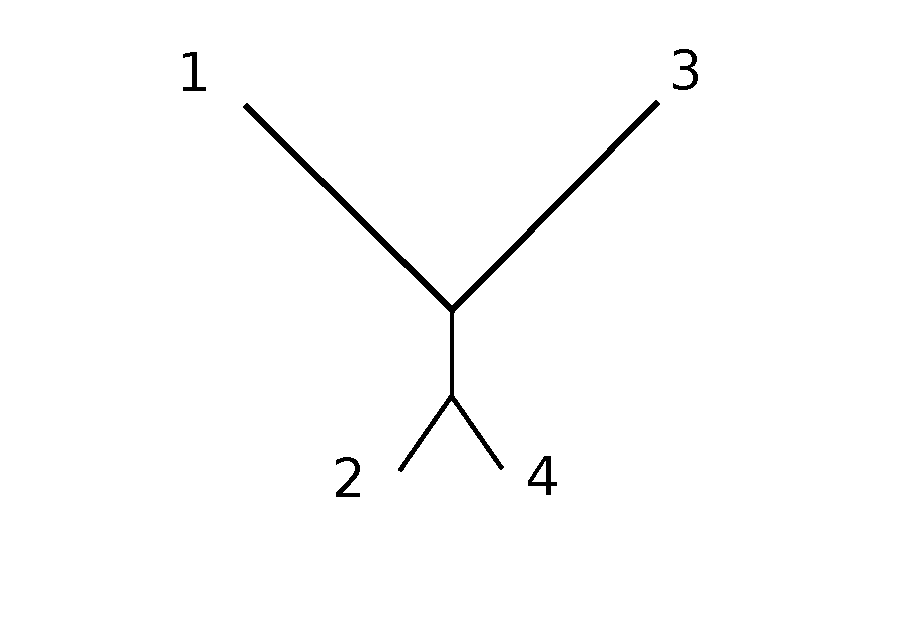
\includegraphics[width=.45\textwidth]{unrooted_farris_tree}
    \caption{Four taxon ``Farris zone'' topology.}
\label{fig:four-taxa-tree}
\end{figure}

Consider the fixed, binary four-tip tree $\tau$ in Fig.~\ref{fig:four-taxa-tree}---this is commonly known as the ``Farris zone'' topology.
The set of all possible character assignments is
\begin{align*}
\mathcal{P}(\{1,2,3,4\}) &= \{\emptyset, \{1,2,3,4\}, \{1\}, \{2,3,4\}, \{2\}, \{1,3,4\}, \{3\}, \{1,2,4\}, \\
                         &\qquad \{1,2\}, \{3,4\}, \{1,3\}, \{2,4\}, \{2,3\}, \{1,4\}, \{1,2,3\}, \{1,4\}\}.
\end{align*}
where each set indicates the tips assigned the character $1$.
For example, $\emptyset$ is the labeling $0000$ and $\{1,3,4\}$ is the labeling $1011$.
Symmetry allows us to group adjacent pairs in $\mathcal{P}(\{1,2,3,4\})$ into equiprobable splits, letting $\siteSplitSet=\{1,2,3\}$.
The unique site splits, collapsing complements, are
\begin{align*}
    \mathcal{P}(\siteSplitSet) &= \{\emptyset, \{1\}, \{2\}, \{3\}, \{1,2\}, \{1,3\}, \{2,3\}, \{1,2,3\}\} \\
& := \{\siteSplit_1, \ldots, \siteSplit_8\}.
\end{align*}
Since we identify character complements, we do not consider the additional splits
\begin{equation*}
\begin{split}
& \mathcal{P}(\{1,2,3,4\}) \setminus \mathcal{P}(\siteSplitSet) = \\
&\qquad \{\{1,2,3,4\}, \{2,3,4\}, \{1,3,4\}, \{1,2,4\}, \{3,4\}, \{2,4\}, \{1,4\}, \{4\}\},
\end{split}
\end{equation*}
the symmetry of the binary character model allowing us to focus only on the elements of $\mathcal{P}(\siteSplitSet)$.
This tree has two internal nodes with $\ancestralSplitSet=\{1,2\}$ and unique ancestral state splits
$$
\mathcal{P}(\ancestralSplitSet) = \{\emptyset, \{1\}, \{2\}, \{1,2\}\}.
$$
Internal node $\{1\}$ is the node connected to leaves $\{1\}$ and $\{3\}$ and internal node $\{2\}$ connected to leaves $\{2\}$ and $\{4\}$.
The mapping from characters to splits in this case will depend on the characters at the tips and the ancestral states.
For example, we take both $\patternToSplit(0000)=\emptyset$ and $\patternToSplit(1111)=\emptyset$.
Similarly, we have $\ancestralToSplit(0000, 00) = \emptyset$ and $\ancestralToSplit(1111, 11)=\emptyset$, needing to take the complement of all the characters present on the tree to identify splits.
As described above we cannot identify complements for ancestral states in the same way as tip states since, for $\siteSplit\in\mathcal{P}(\siteSplitSet)$,
$$
P(\ancestralSplitRV=\emptyset \mid \siteSplitRV=\siteSplit, \tau, t)\neq P(\ancestralSplitRV=\{1,2\} \mid \siteSplitRV=\siteSplit, \tau, t)
$$
in general.

For each site split $\siteSplit\in\mathcal{P}(\siteSplitSet)$, we maximize the likelihood over all $\ancestralSplit\in\mathcal{P}(\ancestralSplitSet)$.
A maximum occurs at one of possibly several ancestral splits in $\mathcal{P}(\ancestralSplitSet)$, defined via $\ancestralSplitPartition_j(\tau, t)$ for the $j$th site split.
As a simple example, say all branch lengths correspond to a probability $p$ ($< 1/2$) of changing character along that branch.
The probabilities of observing ancestral splits for $\siteSplit_1=\emptyset$ are
$$
P(\ancestralSplitRV=\emptyset \mid \siteSplitRV=\emptyset, \tau, t) =
(1-p)^5,
$$
$$
P(\ancestralSplitRV=\{1\} \mid \siteSplitRV=\emptyset, \tau, t) =
P(\ancestralSplitRV=\{2\} \mid \siteSplitRV=\emptyset, \tau, t) =
p^3(1-p)^2,
$$
$$
P(\ancestralSplitRV=\{1,2\} \mid \siteSplitRV=\emptyset, \tau, t) =
p^4(1-p).
$$
%EM Nitpick-- eta takes a tau and a t as arguments. Here we give it a p.
The set of most likely ancestral states contains a single element, here $\ancestralSplitPartition_1(\tau, p)=\{\emptyset\}$.
Then, taking $\xi_1\in\ancestralSplitPartition_1(\tau, p)$ we have
$$
P(\ancestralSplitRV=\xi_1 \mid \siteSplitRV=\emptyset, \tau, t) =
P(\ancestralSplitRV=\emptyset \mid \siteSplitRV=\emptyset, \tau, t) =
(1-p)^5.
$$
For $\siteSplit_5=\{1,2\}$ we have
$$
P(\ancestralSplitRV=\emptyset \mid \siteSplitRV=\{1,2\}, \tau, t) =
P(\ancestralSplitRV=\{1,2\} \mid \siteSplitRV=\{1,2\}, \tau, t) =
p^2(1-p)^3,
$$
$$
P(\ancestralSplitRV=\{1\} \mid \siteSplitRV=\{1,2\}, \tau, t) =
P(\ancestralSplitRV=\{2\} \mid \siteSplitRV=\{1,2\}, \tau, t) =
p^3(1-p)^2.
$$
Here, the set of most likely ancestral states is $\ancestralSplitPartition_5(\tau, p)=\{\emptyset,\{1,2\}\}$, and, for $\xi_5\in\ancestralSplitPartition_5(\tau, p)$,
$$
P(\ancestralSplitRV=\xi_5 \mid \siteSplitRV=\{1,2\}, \tau, t) =
p^2(1-p)^3.
$$

\subsection*{Likelihood computations}

Table~\ref{tab:sitepatprob} contains calculations of site pattern frequencies under these two topologies.
Tables~\ref{tab:farris_likelihoods} and~\ref{tab:fels_likelihoods} contain the values of the likelihood for all possible ancestral states.
Table~\ref{tab:likelihoods} contains calculations of likelihood values for fixed site patterns and topologies that have been maximized over ancestral state patterns.

To compute the likelihood of observing a set of data, we need $P(\ancestralStateColumn=\ancestralSplit_k\mid \alignmentColumn=\siteSplit_j,\tau,t)$ for each $\ancestralSplit_k$ and $\siteSplit_j$.
We remind the reader that the probability of a character change along a branch with fidelity parameter $\theta$ is $(1-\theta)/2$, while the probability of a character remaining the same is $(1+\theta)/2$.
See Fig.~\ref{fig:example_likelihoods} for the parameters on an example site pattern on the Farris tree in Fig.~\ref{fig:farris-fels-top}.
%EM Isn't some of this redundant with the prev paragraph?
Likelihood computations for all site patterns and ancestral states are in Tables~\ref{tab:farris_likelihoods} and~\ref{tab:fels_likelihoods}.
Taking maxima row-wise of each table results in Table~\ref{tab:likelihoods}.

\begin{figure}
\centering
\begin{subfigure}{.45\linewidth}
\centering
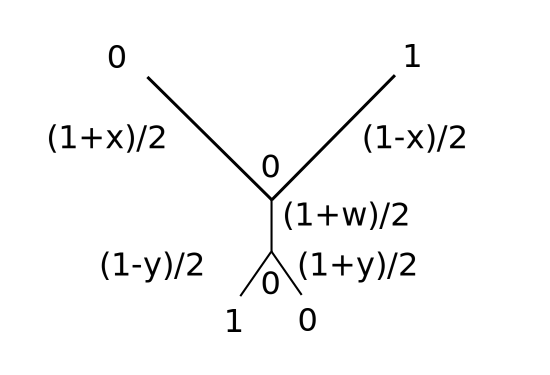
\includegraphics[width=.95\textwidth]{farris_like00}
\caption[short]{}
\end{subfigure}
\begin{subfigure}{.45\linewidth}
\centering
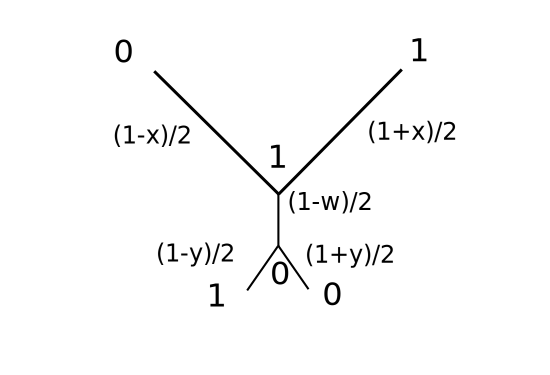
\includegraphics[width=.95\textwidth]{farris_like10}
\caption[short]{}
\end{subfigure}
\caption{
    Example likelihood computations given fidelities $x$, $y$, and $w$.
    In (a), we compute the product to obtain $P(\ancestralStateColumn=\emptyset\mid \alignmentColumn=\{2,3\},\tau_1,t) = (1+x)(1-x)(1+y)(1-y)(1+w)/32$.
    In (b), the same process yields $P(\ancestralStateColumn=\{1\}\mid \alignmentColumn=\{2,3\},\tau_1,t) = (1+x)(1-x)(1+y)(1-y)(1-w)/32$.
}
\label{fig:example_likelihoods}
\end{figure}

\begin{table}
\centering
\begin{tabular}{|l|l|l|}
    \hline
$\siteSplit_j$   &$P(\siteSplitRV=\siteSplit_j \mid \tau_1,t)$&$P(\siteSplitRV=\siteSplit_j \mid \tau_2,t)$\\
    \hline
    $\emptyset$    &$1+x^2+y^2+4xyw+x^2y^2$&$1+2xy+2xyw+x^2w+y^2w+x^2y^2$\\
    $\{1\}$        &$1-x^2+y^2-x^2y^2$&$1-x^2w+y^2w-x^2y^2$\\
    $\{2\}$        &$1+x^2-y^2-x^2y^2$&$1+x^2w-y^2w-x^2y^2$\\
    $\{3\}$        &$1-x^2+y^2-x^2y^2$&$1-x^2w+y^2w-x^2y^2$\\
    $\{1,2\}$      &$1-x^2-y^2+x^2y^2$&$1+2xy-2xyw-x^2w-y^2w+x^2y^2$\\
    $\{1,3\}$      &$1+x^2+y^2-4xyw+x^2y^2$&$1-2xy-2xyw+x^2w+y^2w+x^2y^2$\\
    $\{2,3\}$      &$1-x^2-y^2+x^2y^2$&$1-2xy+2xyw-x^2w-y^2w+x^2y^2$\\
    $\{1,2,3\}$    &$1+x^2-y^2-x^2y^2$&$1+x^2w-y^2w-x^2y^2$\\
    \hline
\end{tabular}
\caption{Site pattern probabilities.
All values are multiplied by $1/8$.}
\label{tab:sitepatprob}
\end{table}

\begin{table}
\centering
\begin{tabular}{|l|ll|}
\multicolumn{3}{c}{$P(\ancestralStateColumn=\ancestralSplit_k\mid \alignmentColumn=\siteSplit_j,\tau_1,t)$}\\
\hline
& \multicolumn{2}{|c|}{$\ancestralSplit_k$}\\
    \hline
    $\siteSplit_j$    &$\emptyset$                                &$\{2\}$  \\
    \hline
     $\emptyset$   &$(1+x)^2   (1+w)(1+y)^2$          &$(1+x)^2   (1-w)(1-y)^2$\\
     $\{1\}$       &$(1+x)(1-x)(1+w)(1+y)^2$          &$(1+x)(1-x)(1-w)(1-y)^2$\\
     $\{2\}$       &$(1+x)^2   (1+w)(1+y)(1-y)$       &$(1+x)^2   (1-w)(1+y)(1-y)$\\
     $\{3\}$       &$(1+x)(1-x)(1+w)(1+y)^2$          &$(1+x)(1-x)(1-w)(1-y)^2$\\
     $\{1,2\}$     &$(1+x)(1-x)(1+w)(1+y)(1-y)$       &$(1+x)(1-x)(1-w)(1+y)(1-y)$\\
     $\{1,3\}$     &$(1-x)^2   (1+w)(1+y)^2$          &$(1-x)^2   (1-w)(1-y)^2$\\
     $\{2,3\}$     &$(1+x)(1-x)(1+w)(1+y)(1-y)$       &$(1+x)(1-x)(1-w)(1+y)(1-y)$\\
     $\{1,2,3\}$   &$(1-x)^2   (1+w)(1+y)(1-y)$       &$(1-x)^2   (1-w)(1+y)(1-y)$\\
    \hline
    \hline
    &$\{1\}$                             &$\{1,2\}$  \\
    \hline
     $\emptyset$   &$(1-x)^2   (1-w)(1+y)^2$     &$(1-x)^2   (1+w)(1-y)^2$\\
     $\{1\}$       &$(1+x)(1-x)(1-w)(1+y)^2$     &$(1+x)(1-x)(1+w)(1-y)^2$\\
     $\{2\}$       &$(1-x)^2   (1-w)(1+y)(1-y)$  &$(1-x)^2   (1+w)(1+y)(1-y)$\\
     $\{3\}$       &$(1+x)(1-x)(1-w)(1+y)^2$     &$(1+x)(1-x)(1+w)(1-y)^2$\\
     $\{1,2\}$     &$(1+x)(1-x)(1-w)(1+y)(1-y)$  &$(1+x)(1-x)(1+w)(1+y)(1-y)$\\
     %EM I was doing some spot-checking here, and this line seems strange.
     %EM I'd think that this left hand entry has everything in the upper half of the tree in the "on" state, which means that it should be (1+x)^2   (1-w)(1+y)^2, no?
     %das: looks like I was silly and was computing {2,4} instead of {1,3}. Luckily it doesn't change anything. Did same with {4} and {1,2,3}...
     $\{1,3\}$     &$(1+x)^2   (1-w)(1+y)^2$     &$(1+x)^2   (1+w)(1-y)^2$\\
     $\{2,3\}$     &$(1+x)(1-x)(1-w)(1+y)(1-y)$  &$(1+x)(1-x)(1+w)(1+y)(1-y)$\\
     $\{1,2,3\}$   &$(1+x)^2   (1-w)(1+y)(1-y)$  &$(1+x)^2   (1+w)(1+y)(1-y)$\\
    \hline
\end{tabular}
\caption{Likelihood calculations for all site patterns and internal states of the Farris tree.
All values multiplied by $1/32$.}
\label{tab:farris_likelihoods}
\end{table}

\begin{table}
\centering
\begin{tabular}{|l|ll|}
\multicolumn{3}{c}{$P(\ancestralStateColumn=\ancestralSplit_k\mid \alignmentColumn=\siteSplit_j,\tau_2,t)$}\\
\hline
& \multicolumn{2}{|c|}{$\ancestralSplit_k$}\\
    \hline
    $\siteSplit_j$    &$\emptyset$                                &$\{2\}$  \\
    \hline
     $\emptyset$   &$(1+x)^2   (1+w)(1+y)^2$           &$(1+x)(1-x)(1-w)(1+y)(1-y)$\\
     $\{1\}$       &$(1+x)(1-x)(1+w)(1+y)^2$           &$(1-x)^2   (1-w)(1+y)(1-y)$\\
     $\{2\}$       &$(1+x)^2   (1+w)(1+y)(1-y)$        &$(1+x)(1-x)(1-w)(1-y)^2$\\
     $\{3\}$       &$(1+x)(1-x)(1+w)(1+y)^2$           &$(1+x)^2   (1-w)(1+y)(1-y)$\\
     %das: looks also like I did the complement of the ancestral states for {1,2} and {2,3} here by accident. Still doesn't change anything afaik
     %das: All that happened was entries swapped row-wise, which wouldn't affect taking a maximum or summing.
     $\{1,2\}$     &$(1+x)(1-x)(1+w)(1+y)(1-y)$        &$(1-x)^2   (1-w)(1-y)^2$\\
     $\{1,3\}$     &$(1-x)^2   (1+w)(1+y)^2$           &$(1+x)(1-x)(1-w)(1+y)(1-y)$\\
     $\{2,3\}$     &$(1+x)(1-x)(1+w)(1+y)(1-y)$        &$(1+x)^2   (1-w)(1-y)^2$\\
     $\{1,2,3\}$   &$(1-x)^2   (1+w)(1+y)(1-y)$        &$(1+x)(1-x)(1-w)(1-y)^2$\\
    \hline
    \hline
    &$\{1\}$                             &$\{1,2\}$  \\
    \hline
     $\emptyset$   &$(1+x)(1-x)(1-w)(1+y)(1-y)$        &$(1-x)^2   (1+w)(1-y)^2$\\
     $\{1\}$       &$(1+x)^2   (1-w)(1+y)(1-y)$        &$(1+x)(1-x)(1+w)(1-y)^2$\\
     $\{2\}$       &$(1+x)(1-x)(1-w)(1+y)^2$           &$(1-x)^2   (1+w)(1+y)(1-y)$\\
     $\{3\}$       &$(1-x)^2   (1-w)(1+y)(1-y)$        &$(1+x)(1-x)(1+w)(1-y)^2$\\
     $\{1,2\}$     &$(1+x)^2   (1-w)(1+y)^2$           &$(1+x)(1-x)(1+w)(1+y)(1-y)$\\
     $\{1,3\}$     &$(1+x)(1-x)(1-w)(1+y)(1-y)$        &$(1+x)^2   (1+w)(1-y)^2$\\
     $\{2,3\}$     &$(1-x)^2   (1-w)(1+y)^2$           &$(1+x)(1-x)(1+w)(1+y)(1-y)$\\
     $\{1,2,3\}$   &$(1+x)(1-x)(1-w)(1+y)^2$           &$(1+x)^2   (1+w)(1+y)(1-y)$\\
\hline
\end{tabular}
\caption{Likelihood calculations for all site patterns and internal states of Felsenstein tree.
All values multiplied by $1/32$.}
\label{tab:fels_likelihoods}
\end{table}

\begin{table}
\centering
\begin{tabular}{|l|ll|}
    \multicolumn{3}{c}{$\tau=\tau_1$}\\
    \hline
    $\siteSplit_j$    & $\ancestralSplitPartition_j(\tau, t)$ & $P(\ancestralSplitRV=\xi_j \mid \siteSplitRV=\siteSplit_j,\tau,t)$\\
    \hline
    $\emptyset$&
    $\emptyset$&
    $(1+x)^2   (1+w)(1+y)^2$\\
     $\{1\}$    &
    $\emptyset$&
    $(1+x)(1-x)(1+w)(1+y)^2$\\
     $\{2\}$    &
    $\emptyset$&
    $(1+x)^2   (1+w)(1+y)(1-y)$\\
     $\{3\}$    &
    $\emptyset$&
    $(1+x)(1-x)(1+w)(1+y)^2$\\
    $\{1,2\}$  &
    $\{\emptyset,\{1,2\}\}$&
    $(1+x)(1-x)(1+w)(1+y)(1-y)$\\
    $\{1,3\}$  &
    $\left\{\begin{array}{l}
                    \emptyset\\
                    \{1\}\\
                    \{1,2\}
                \end{array}\right.$&
    $\begin{array}{l}
                    (1-x)^2   (1+w)(1+y)^2\\
                    (1+x)^2   (1-w)(1+y)^2\\
                    (1+x)^2   (1+w)(1-y)^2
                \end{array}$\\
    $\{2,3\}$  &
                $\{\emptyset,\{1,2\}\}$&
                $(1+x)(1-x)(1+w)(1+y)(1-y)$\\
    $\{1,2,3\}$&
                $\{1,2\}$&
                $(1+x)^2   (1+w)(1+y)(1-y)$\\
    \hline
    \multicolumn{3}{c}{$\tau=\tau_2$}\\
    \hline
    $\siteSplit_j$    & $\ancestralSplitPartition_j(\tau, t)$ & $P(\ancestralSplitRV=\xi_j \mid \siteSplitRV=\siteSplit_j,\tau,t)$\\
    \hline
    $\emptyset$       &$\emptyset$&$(1+x)^2   (1+w)(1+y)^2$\\
    $\{1\}$          &
    $\left\{\begin{array}{l}
                    \emptyset\\
                    \{1\}
                \end{array}\right.$&
    $\begin{array}{l}
                        (1+x)(1-x)(1+w)(1+y)^2\\
                        (1+x)^2   (1-w)(1+y)(1-y)
                    \end{array}$\\
      $\{2\}$          &
    $\left\{\begin{array}{l}
                    \emptyset\\
                    \{1\}
                \end{array}\right.$&
    $\begin{array}{l}
                    (1+x)^2   (1+w)(1+y)(1-y)\\
                    (1+x)(1-x)(1-w)(1+y)^2
                    \end{array}$\\
      $\{3\}$          &
    $\left\{\begin{array}{l}
                    \emptyset\\
                    \{2\}
                \end{array}\right.$&
    $\begin{array}{l}
                    (1+x)(1-x)(1+w)(1+y)^2\\
                    (1+x)^2   (1-w)(1+y)(1-y)
                    \end{array}$\\
     $\{1,2\}$         &
    $\left\{\begin{array}{l}
                    \{\emptyset,\{1,2\}\}\\
                    \{1\}
                \end{array}\right.$&
    $\begin{array}{l}
                    (1+x)(1-x)(1+w)(1+y)(1-y)\\
                    (1+x)^2   (1-w)(1+y)^2
                    \end{array}$\\
     $\{1,3\}$         &
    $\left\{\begin{array}{l}
                    \emptyset\\
                    \{\{1\},\{2\}\}\\
                    \{1,2\}
                \end{array}\right.$&
    $\begin{array}{l}
                    (1-x)^2   (1+w)(1+y)^2\\
                    (1+x)(1-x)(1-w)(1+y)(1-y)\\
                    (1+x)^2   (1+w)(1-y)^2
                    \end{array}$\\
      $\{2,3\}$        &
    $\left\{\begin{array}{l}
                    \{\emptyset,\{1,2\}\}\\
                    \{1\}\\
                    \{2\}
                \end{array}\right.$&
    $\begin{array}{l}
                    (1+x)(1-x)(1+w)(1+y)(1-y)\\
                    (1-x)^2   (1-w)(1+y)^2\\
                    (1+x)^2   (1-w)(1-y)^2
                    \end{array}$\\
     $\{1,2,3\}$       &
    $\left\{\begin{array}{l}
                    \{2\} \\
                    \{1,2\}
                \end{array}\right.$&
    $\begin{array}{l}
                    (1+x)(1-x)(1-w)(1+y)^2 \\
                    (1+x)^2   (1+w)(1+y)(1-y)
                    \end{array}$\\
    \hline
\end{tabular}
\caption{Likelihood calculations for all site patterns and ancestral state partitions.
All values multiplied by $1/32$.
Likelihoods with multiple entries have maxima determined by unknown branch length parameters.
See Appendix for full calculations.}
\label{tab:likelihoods}
\end{table}

\subsection*{Form of the likelihood}

Consider the Farris tree with arbitrary branch lengths, i.e., $\tilde{t}=\{x_1,y_1,x_2,y_2,w\}$.
We now show that, in the case of the Farris tree, exchanging $x_1$ with $x_2$ and $y_1$ with $y_2$ does not change the value of the likelihood, and that fixing both the top two branch lengths to be equal and the bottom two branch lengths to be equal will obtain the same maximum likelihood estimate as in the case of arbitrary branch lengths.
Using the Hadamard transform approach, we calculate the generating probabilities on the Farris tree.
For site split $\emptyset$,
\begin{align*}
    P(\siteSplitRV=\emptyset\mid \tau_1, \tilde{t}) & = \frac{1}{8} (1 + x_1x_2 +  y_1y_2 +  x_1y_1w + x_1y_2w + y_1x_2w + x_2y_2w + x_1y_1x_2y_2) \\
                                              & = \frac{1}{8} (1 + x_1x_2 +  y_1y_2 +  w[x_1y_1 + x_1y_2 + y_1x_2 + x_2y_2] + x_1y_1x_2y_2) \\
                                              & = \frac{1}{8} (1 + x_1x_2 +  y_1y_2 +  w[x_1 + x_2][y_1 + y_2] + x_1y_1x_2y_2).
\end{align*}
and this probability is unchanged when $x_1$ is exchanged with $x_2$ and $y_1$ is exchanged with $y_2$.
All other generating probabilities will differ only in the signs of each term.
For example, for site split $\{1\}$ we have
\begin{align*}
    P(\siteSplitRV=\{1\}\mid \tau_1, \tilde{t}) & = \frac{1}{8} (1 - x_1x_2 +  y_1y_2 +  w[-x_1 + x_2][y_1 + y_2] - x_1y_1x_2y_2)
\end{align*}
and for site split $\{3\}$ we have
\begin{align*}
    P(\siteSplitRV=\{3\}\mid \tau_1, \tilde{t}) & = \frac{1}{8} (1 - x_1x_2 +  y_1y_2 +  w[x_1 - x_2][y_1 + y_2] - x_1y_1x_2y_2)
\end{align*}
meaning if we exchange the values of $x_1$ and $x_2$ then these probabilities swap values.
The corresponding possibilities for the likelihood values are
\begin{align*}
    P(\ancestralSplitRV=\emptyset \mid \siteSplitRV=\{1\}, \tau_1, \tilde{t}) &= \frac{1}{32}(1-x_1)(1+x_2)(1+w)(1+y_1)(1+y_2); \\
    P(\ancestralSplitRV=\{1\} \mid \siteSplitRV=\{1\}, \tau_1, \tilde{t}) &= \frac{1}{32}(1+x_1)(1-x_2)(1-w)(1+y_1)(1+y_2); \\
    P(\ancestralSplitRV=\{2\} \mid \siteSplitRV=\{1\}, \tau_1, \tilde{t}) &= \frac{1}{32}(1-x_1)(1+x_2)(1-w)(1-y_1)(1-y_2); \\
    P(\ancestralSplitRV=\{1,2\} \mid \siteSplitRV=\{1\}, \tau_1, \tilde{t}) &= \frac{1}{32}(1+x_1)(1-x_2)(1+w)(1-y_1)(1-y_2);
\end{align*}
for site split $\{1\}$ and
\begin{align*}
        P(\ancestralSplitRV=\emptyset \mid \siteSplitRV=\{3\}, \tau_1, \tilde{t}) &= \frac{1}{32}(1+x_1)(1-x_2)(1+w)(1+y_1)(1+y_2); \\
    P(\ancestralSplitRV=\{1\} \mid \siteSplitRV=\{3\}, \tau_1, \tilde{t}) &= \frac{1}{32}(1-x_1)(1+x_2)(1-w)(1+y_1)(1+y_2); \\
    P(\ancestralSplitRV=\{2\} \mid \siteSplitRV=\{3\}, \tau_1, \tilde{t}) &= \frac{1}{32}(1+x_1)(1-x_2)(1-w)(1-y_1)(1-y_2); \\
    P(\ancestralSplitRV=\{1,2\} \mid \siteSplitRV=\{3\}, \tau_1, \tilde{t}) &= \frac{1}{32}(1-x_1)(1+x_2)(1+w)(1-y_1)(1-y_2);
\end{align*}
for site split $\{3\}$, which also both swap values when $x_1$ and $x_2$ are exchanged.

The same can be done for the splits $\{2\}$ and $\{1,2,3\}$ by exchanging $y_1$ and $y_2$ as well as $\{1,2\}$ and $\{1,3\}$ by exchanging both $x_1$ with $x_2$ and $y_1$ with $y_2$.
The split $\{1,3\}$ is unchanged by exchanging $x_1$ with $x_2$ and $y_1$ with $y_2$.

Since exchanging $x_1$ and $x_2$ does not change the value of the log-likelihood $\ell_{\tau_1,t^*}(\tau_1, \tilde{t}; \fullAncestralSplitPartitions(\tau_1,\tilde{t}))$, $x_1=x_2$ at the maximum.
The analogous statement holds for $y_1$ and $y_2$.
The Felsenstein tree does not admit this property, but, since we are interested in a lower bound for this tree, we simplify the objective function by constraining $x_1=x_2$ and $y_1=y_2$ similarly.

\subsection*{Theorems and proofs}

%EM Here we are restating.
\topoInconsist*

\begin{proof}
In general,
$$
\max_{t} \ \ell_{\tau^*,t^*}(\tau, t; \fullAncestralSplitPartitions(\tau,t)) \le
    \shannonDivergence_{\tau^*,t^*}(\tau^*,t^*)
    + \tilde{\ell}_{\tau^*,t^*}(\tau, \hat{t}; \fullAncestralSplitPartitions(\tau, \hat{t}))
$$
is an upper bound for the joint maximum of \eqref{eq:log_likelihood_simplified} using Gibbs's inequality
$$
\shannonDivergence_{\tau^*,t^*}(\tau,t) \le \shannonDivergence_{\tau^*,t^*}(\tau^*,t^*)
$$
and
$$
\hat{t} = \argmax_{t} \ \tilde{\ell}_{\tau^*,t^*}(\tau, t; \fullAncestralSplitPartitions(\tau,t)).
$$
Similarly,
$$
\max_{t} \ \ell_{\tau^*,t^*}(\tau, t; \fullAncestralSplitPartitions(\tau,t)) \ge
    \shannonDivergence_{\tau^*,t^*}(\tau,\hat{t})
    + \tilde{\ell}_{\tau^*,t^*}(\tau, \hat{t}; \fullAncestralSplitPartitions(\tau, \hat{t}))
$$
is a lower bound.

Assume $\tau^*=\tau_1$.
Following \eqref{eq:hadamard_probability}, let
$$
p_{\emptyset} := p_{\emptyset}(x^*, y^*) = P(\siteSplitRV=\emptyset \mid \tau=\tau_1,t=t^*),
$$
with similar definitions for the remaining generating probabilities.
The full Farris tree log-likelihood takes one of three values depending on branch lengths, which is due to site split $\{1,3\}$ (see Table~\ref{tab:likelihoods} for $\tau = \tau_1$).
We begin by writing out the case for the ancestral state split $\{1\}$.
Directly substituting in \eqref{eq:site_pattern_likelihood}, the log-likelihood is
\begin{align}
    \label{eq:farris_likelihood}
    \ell_{\tau_1,t^*}(\tau_1, t; \fullAncestralSplitPartitions(\tau_1,t))
    &=        p_{\emptyset}  \cdot\log(1+x^2+y^2+4xyw+x^2y^2) \nonumber \\
    &\qquad + p_{1}          \cdot\log(1-x^2+y^2-x^2y^2) \nonumber \\
    &\qquad + p_{2}          \cdot\log(1+x^2-y^2-x^2y^2) \nonumber \\
    &\qquad + p_{3}          \cdot\log(1-x^2+y^2-x^2y^2) \nonumber \\
    &\qquad + p_{12}         \cdot\log(1-x^2-y^2+x^2y^2) \nonumber \\
    &\qquad + p_{13}         \cdot\log(1+x^2+y^2-4xyw+x^2y^2) \nonumber \\
    &\qquad + p_{23}         \cdot\log(1-x^2-y^2+x^2y^2) \nonumber \\
    &\qquad + p_{123}        \cdot\log(1+x^2-y^2-x^2y^2) \nonumber \\
    &\qquad - \log(8) \nonumber \\
    &\qquad + p_{\emptyset}  \cdot\log((1+x)^2   (1+w)(1+y)^2) \nonumber \\
    &\qquad + p_{1}          \cdot\log((1+x)(1-x)(1+w)(1+y)^2) \nonumber \\
    &\qquad + p_{2}          \cdot\log((1+x)^2   (1+w)(1+y)(1-y)) \nonumber \\
    &\qquad + p_{3}          \cdot\log((1+x)(1-x)(1+w)(1+y)^2) \nonumber \\
    &\qquad + p_{12}         \cdot\log((1+x)(1-x)(1+w)(1+y)(1-y)) \nonumber \\
    &\qquad + p_{13}         \cdot\log((1+x)^2   (1-w)(1+y)^2) \nonumber \\
    &\qquad + p_{23}         \cdot\log((1+x)(1-x)(1+w)(1+y)(1-y)) \nonumber \\
    &\qquad + p_{123}        \cdot\log((1+x)^2   (1+w)(1+y)(1-y)).
\end{align}
We use the facts that, for $x,y\in[0,1]$,
\begin{align*}
1-x^2+y^2-x^2y^2 & = (1+x)(1-x)(1+y^2) \le (1+x)(1-x)(1+y) \\
1+x^2-y^2-x^2y^2 & = (1+x^2)(1+y)(1-y) \le (1+x)(1+y)(1-y) \\
1+x^2+y^2+x^2y^2 & = (1+x^2)(1+y^2) \le (1+x)(1+y) \\
4xy & = 2x \cdot 2y \le (1+x^2)(1+y^2) \le (1+x)(1+y).
\end{align*}
The term $p_{\emptyset}$ is bounded as
\begin{align*}
    p_{\emptyset} & = \log(1+x^2+y^2+4xyw+x^2y^2) \\
                  & \le \log(1+x^2+y^2+4xy+x^2y^2) \\
                  & \le \log(2(1+x)(1+y))
\end{align*}
and $p_{13}$ is bounded as
\begin{align*}
    p_{13} & = \log(1+x^2+y^2-4xyw+x^2y^2) \\
                  & \le \log(1+x^2+y^2+x^2y^2) \\
                  & \le \log((1+x)(1+y)).
\end{align*}
Factoring and making these substitutions results in
\begin{align*}
&    \ell_{\tau_1,t^*}(\tau_1, t; \fullAncestralSplitPartitions(\tau_1,t)) \\
&\qquad \le      p_{\emptyset}  \cdot\log(2(1+x)(1+y))
+ p_{1}          \cdot\log((1+x)(1-x)(1+y)) \\
    &\qquad\qquad + p_{2}          \cdot\log((1+x)(1+y)(1-y))
+ p_{3}          \cdot\log((1+x)(1-x)(1+y)) \\
    &\qquad\qquad + p_{12}         \cdot\log((1+x)(1-x)(1+y)(1-y))
+ p_{13}         \cdot\log((1+x)(1+y)) \\
    &\qquad\qquad + p_{23}         \cdot\log((1+x)(1-x)(1+y)(1-y))
+ p_{123}        \cdot\log((1+x)(1+y)(1-y))
- \log(8) \\
    &\qquad\qquad + p_{\emptyset}  \cdot\log((1+x)^2   (1+w)(1+y)^2)
+ p_{1}          \cdot\log((1+x)(1-x)(1+w)(1+y)^2) \\
    &\qquad\qquad + p_{2}          \cdot\log((1+x)^2   (1+w)(1+y)(1-y))
+ p_{3}          \cdot\log((1+x)(1-x)(1+w)(1+y)^2) \\
    &\qquad\qquad + p_{12}         \cdot\log((1+x)(1-x)(1+w)(1+y)(1-y))
+ p_{13}         \cdot\log((1+x)^2   (1-w)(1+y)^2) \\
    &\qquad\qquad + p_{23}         \cdot\log((1+x)(1-x)(1+w)(1+y)(1-y))
+ p_{123}        \cdot\log((1+x)^2   (1+w)(1+y)(1-y)) \\
&\qquad =      p_{\emptyset}  \cdot\log(2)
+ \log(1+x)
+ (p_{1}+p_{3}+p_{12}+p_{23})\cdot\log(1-x) \\
&\qquad\qquad + \log(1+y)
+ (p_{2}+p_{12}+p_{23}+p_{123})\cdot\log(1-y) \\
&\qquad\qquad + (2-p_{1}-p_{3}-p_{12}-p_{23})\cdot\log(1+x)
+ (p_{1}+p_{3}+p_{12}+p_{23})\cdot\log(1-x) \\
&\qquad\qquad + (2-p_{2}-p_{12}-p_{23}-p_{123})\cdot\log(1+y)
+ (p_{2}+p_{12}+p_{23}+p_{123})\cdot\log(1-y) \\
&\qquad\qquad + (1-p_{13})\cdot\log(1+w)
+ p_{13}\cdot\log(1-w)
- \log(8) \\
&\qquad =      p_{\emptyset}  \cdot\log(2)
+ (3-p_{1}-p_{3}-p_{12}-p_{23})\cdot\log(1+x)
+ 2(p_{1}+p_{3}+p_{12}+p_{23})\cdot\log(1-x) \\
&\qquad\qquad + (3-p_{2}-p_{12}-p_{23}-p_{123})\cdot\log(1+y)
+ 2(p_{2}+p_{12}+p_{23}+p_{123})\cdot\log(1-y) \\
&\qquad\qquad + (1-p_{13})\cdot\log(1+w)
+ p_{13}\cdot\log(1-w)
- \log(8).
\end{align*}
To simplify, let
\begin{equation}
    \begin{aligned}
        a_{1} &= 3-p_{1}-p_{3}-p_{12}-p_{23}, \\
        a_{2} &= 2(p_{1}+p_{3}+p_{12}+p_{23}), \\
        a_{3} &= 3-p_{2}-p_{12}-p_{23}-p_{123}, \\
        a_{4} &= 2(p_{2}+p_{12}+p_{23}+p_{123}), \\
    \end{aligned}
    \label{eq:a_const}
\end{equation}
so that
\begin{equation*}
\begin{split}
&    \ell_{\tau_1,t^*}(\tau_1, t; \fullAncestralSplitPartitions(\tau_1,t)) \\
&\qquad \le      p_{\emptyset}  \cdot\log(2)
+ a_{1}\cdot\log(1+x)
+ a_{2}\cdot\log(1-x)
+ a_{3}\cdot\log(1+y) \\
&\qquad\qquad + a_{4}\cdot\log(1-y)
+ (1-p_{13})\cdot\log(1+w)
+ p_{13}\cdot\log(1-w)
- \log(8).
\end{split}
\end{equation*}
Maximizing over the unknown terms yields
$$
\hat{x} = \frac{a_{1}-a_{2}}{a_{1}+a_{2}}, \ \hat{y} = \frac{a_{3}-a_{4}}{a_{3}+a_{4}}, \ \hat{w} = 1-2p_{13}.
$$
Trivially $0 \le \hat{w} \le 1$.
We check that $0 \le \hat{x} \le 1$ and $0 \le \hat{y} \le 1$ so these maximizers are valid.
Letting
$$
\tilde{p} = p_{1}+p_{3}+p_{12}+p_{23}
$$
we have
$$
\hat{x} = \frac{3-\tilde{p} - 2\tilde{p}}{3-\tilde{p}+2\tilde{p}} = \frac{3-3\tilde{p}}{3+\tilde{p}},
$$
and, since $0 \le \tilde{p} \le 1/2$, $0 \le \hat{x} \le 1$.
The same approach works for $\hat{y}$.
The upper bound for the likelihood is then maximized at
\begin{align*}
&    \ell_{\tau_1,t^*}(\tau_1, t; \fullAncestralSplitPartitions(\tau_1,t)) \\
&\qquad\le      p_{\emptyset}  \cdot\log(2)
+ a_{1}\cdot\log\frac{2a_{1}}{a_{1}+a_{2}}
+ a_{2}\cdot\log\frac{2a_{2}}{a_{1}+a_{2}}
+ a_{3}\cdot\log\frac{2a_{3}}{a_{3}+a_{4}} \\
&\qquad\qquad + a_{4}\cdot\log\frac{2a_{4}}{a_{3}+a_{4}}
+ (1-p_{13})\cdot\log(2(1-p_{13}))
+ p_{13}\cdot\log(2p_{13})
- \log(8) \\
&\qquad := C^{1}_{\tau_1,\tau_1}(x^*, y^*).
\end{align*}

The other two possible ancestral state splits for the likelihood of the site split $\{1,3\}$ admit similar simplifications.
Call
\begin{equation}
    \begin{aligned}
        a_{1}' &= a_{1}-2p_{13}, \\
        a_{2}' &= a_{2}+2p_{13}, \\
        a_{3}' &= a_{3}-2p_{13}, \\
        a_{4}' &= a_{4}+2p_{13}. \\
    \end{aligned}
    \label{eq:a_const_prime}
\end{equation}
We also now need to check that
$$
\hat{x} = \frac{a_{1}'-a_{2}'}{a_{1}'+a_{2}'}, \ \hat{y} = \frac{a_{3}'-a_{4}'}{a_{3}'+a_{4}'}
$$
are both between zero and one.
It will suffice to show
$$
0 \le \tilde{p} - 2p_{13} \le 1
$$
and
$$
0 \le \tilde{p} + 2p_{13} \le 1
$$
for $\tilde{p}$ defined above, which is equivalent to showing $p_{13} \le 1/4$.
Using Table~\ref{tab:sitepatprob} and $t^*$,
$$
p_{13} = \frac{1}{8}\left(1 + (x^*)^2 + (y^*)^2 - 4x^*(y^*)^2 + (x^*)^2(y^*)^2\right).
$$
We see that
$$
1 + (x^*)^2 + (y^*)^2 - 4x^*(y^*)^2 + (x^*)^2(y^*)^2 \le 2 \iff (y^*)^2\left(1 - 4x^* + (x^*)^2\right) \le 1 - (x^*)^2
$$
and
$$
(y^*)^2\left(1 - 4x^* + (x^*)^2\right) \le 1 - 4x^* + (x^*)^2 \le 1 - (x^*)^2,
$$
the last inequality holding if $x^* \le 2$.
Thus, $p_{13} \le 2/8 = 1/4$ and our $\hat{x}$ and $\hat{y}$ are valid.

To bound the case of $\ancestralSplitPartition_j(\tau_1, t) = \emptyset$,
\begin{align*}
&    \ell_{\tau_1,t^*}(\tau_1, t; \fullAncestralSplitPartitions(\tau_1,t)) \\
&\qquad\le      p_{\emptyset}  \cdot\log(2)
+ a_{1}'\cdot\log\frac{2a_{1}'}{a_{1}'+a_{2}'}
+ a_{2}'\cdot\log\frac{2a_{2}'}{a_{1}'+a_{2}'} \\
&\qquad\qquad + a_{3}\cdot\log\frac{2a_{3}}{a_{3}+a_{4}}
+ a_{4}\cdot\log\frac{2a_{4}}{a_{3}+a_{4}}
+ \log(2)
- \log(8) \\
&\qquad := C^{2}_{\tau_1,\tau_1}(x^*, y^*),
\end{align*}
and, for the case of $\ancestralSplitPartition_j(\tau_1, t) = \{1,2\}$,
\begin{align*}
&    \ell_{\tau_1,t^*}(\tau_1, t; \fullAncestralSplitPartitions(\tau_1,t)) \\
&\qquad\le      p_{\emptyset}  \cdot\log(2)
+ a_{1}\cdot\log\frac{2a_{1}}{a_{1}+a_{2}}
+ a_{2}\cdot\log\frac{2a_{2}}{a_{1}+a_{2}} \\
&\qquad\qquad+ a_{3}'\cdot\log\frac{2a_{3}'}{a_{3}'+a_{4}'}
+ a_{4}'\cdot\log\frac{2a_{4}'}{a_{3}'+a_{4}'}
+ \log(2)
- \log(8) \\
&\qquad := C^{3}_{\tau_1,\tau_1}(x^*, y^*).
\end{align*}
All bounds are functions only of $x,y$ through the true generating probabilities $x^*, y^*$.
Call the upper bound
$$
C_0(x^*, y^*) := \max\left(C^{1}_{\tau_1,\tau_1}(x^*, y^*), C^{2}_{\tau_1,\tau_1}(x^*, y^*), C^{3}_{\tau_1,\tau_1}(x^*, y^*)\right).
$$

We construct a similar lower bound on the Felsenstein tree partial likelihood.
In the Felsenstein case, there are various optimal internal states depending on branch lengths (Table~\ref{tab:likelihoods}; $\tau = \tau_2$).
We can bound these below replacing $1+w$ with $1-w$ as follows.
For the site split $\{1,2\}$, we would like to find a lower bound for
$$
\max\left((1+x)^2 (1-w)(1+y)^2, (1+x)(1-x)(1+w)(1+y)(1-y)\right).
$$
We observe that
$$
(1+x)^2 (1-w)(1+y)^2 > (1+x)(1-x)(1-w)(1+y)(1-y)
$$
always, and thus the maximum can be bounded below by $(1+x)^2 (1-w)(1+y)^2$.
For the other site splits we consider two cases.
If $(1+x)(1-y) > (1-x)(1+y)$, then
$$
(1+x)^2(1-w)(1+y)(1-y) > (1+x)(1-x)(1-w)(1+y)^2
$$
meaning the cases $\{1\}, \{2\}, \{3\}$ and $\{1,2,3\}$ will have likelihoods bounded below by
$$
(1+x)^2(1-w)(1+y)(1-y).
$$
For the cases $\{1,3\}$ and $\{2,3\}$ and the same condition, we have
$$
(1+x)^2(1-w)(1-y)^2 > (1-x)^2(1-w)(1+y)^2
$$
and
$$
(1+x)^2(1-w)(1-y)^2 > (1+x)(1-x)(1-w)(1+y)(1-y),
$$
yielding lower bounds of
$$
(1+x)^2(1-w)(1-y)^2
$$
in these cases.
The full likelihood in this case is then bounded below by
\begin{align*}
    \tilde{\ell}_{\tau_1,t^*}(\tau_2, t; \fullAncestralSplitPartitions(\tau_2,t))
    &\ge      p_{\emptyset}  \cdot\log((1+x)^2   (1-w)(1+y)^2) \\
    &\qquad + p_{1}          \cdot\log((1+x)^2   (1-w)(1+y)(1-y)) \\
    &\qquad + p_{2}          \cdot\log((1+x)^2   (1-w)(1+y)(1-y)) \\
    &\qquad + p_{3}          \cdot\log((1+x)^2   (1-w)(1+y)(1-y)) \\
    &\qquad + p_{12}         \cdot\log((1+x)^2   (1-w)(1+y)^2) \\
    &\qquad + p_{123}        \cdot\log((1+x)^2   (1-w)(1+y)(1-y))\\
    &\qquad + p_{13}         \cdot\log((1+x)^2   (1-w)(1-y)^2) \\
    &\qquad + p_{23}         \cdot\log((1+x)^2   (1-w)(1-y)^2).
\end{align*}
When $(1+x)(1-y) < (1-x)(1+y)$, similar arguments yield the lower bound
\begin{align*}
    \tilde{\ell}_{\tau_1,t^*}(\tau_2, t; \fullAncestralSplitPartitions(\tau_2,t))
    &\ge      p_{\emptyset}  \cdot\log((1+x)^2    (1-w)(1+y)^2) \\
    &\qquad + p_{1}          \cdot\log((1+x)(1-x)(1-w)(1+y)^2) \\
    &\qquad + p_{2}          \cdot\log((1+x)(1-x)(1-w)(1+y)^2) \\
    &\qquad + p_{3}          \cdot\log((1+x)(1-x)(1-w)(1+y)^2) \\
    %See above.
    &\qquad + p_{12}         \cdot\log((1+x)^2    (1-w)(1+y)^2) \\
    &\qquad + p_{123}        \cdot\log((1+x)(1-x)(1-w)(1+y)^2)\\
    &\qquad + p_{13}         \cdot\log((1-x)^2    (1-w)(1+y)^2) \\
    &\qquad + p_{23}         \cdot\log((1-x)^2    (1-w)(1+y)^2).
\end{align*}
Letting
$$
b = p_{1}+p_{2}+p_{3}+p_{123}
$$
yields
$$
    \tilde{\ell}_{\tau_1,t^*}(\tau_2, t; \fullAncestralSplitPartitions(\tau_2,t))
    \ge      2\cdot\log(1+x)
    + (2-b)  \cdot\log(1+y)
    + b      \cdot\log(1-y)
    + \log(1-w)
$$
for the first lower bound, and we get the equivalent expression for the second lower bound by exchanging $x$ and $y$.
Maximizing either lower bound over $t$, we obtain
$$
\tilde{\ell}_{\tau_1,t^*}(\tau_2, t; \fullAncestralSplitPartitions(\tau_2,t))
\ge      2\cdot\log(2)
+ (2-b)  \cdot\log(2-b)
+ b      \cdot\log(b)
$$
%EM Shouldn't this be 2p_{\emptyset}-1 ? It doesn't matter for the bound, but...
%das If we call p_{\emptyset} just p, we're maximizing
%   p log (1 + w) + (1 - p) log (1 - w).
%As before, a_1 log(1+x) + a_2 log(1-x) is maximized at x = (a_1 - a_2) / (a_1 + a_2).
%So then w = (p - (1 - p)) / (p + (1 - p)) = (2p - 1) / 1 = 2p - 1.
%So you're right. Good catch.
%
%Unfortunately, I realized the above does not work for us since 2p - 1 is not guaranteed to be between 0 and 1, as x should be (see the stuff I added justifying this above).
%Rather than do a constrained optimization, I just bounded the p_{\emptyset}\log(1+w) term below by p_{\emptyset}\log(1-w).
i.e.\ the maximum is achieved at $\{1,1-b,0\}$.
Our lower bound is
$$
C_1(x^*, y^*) := \shannonDivergence_{\tau_1,t^*}(\tau_2,\{1,1-b,0\}) + 2\cdot\log(2) + (2-b)\cdot\log(2-b) + b\cdot\log(b).
$$
See Fig.~\ref{fig:inconsistency-farris} for the values of $0 < x^*, y^* < 1$ where $C_1(x^*, y^*) > C_0(x^*, y^*)$ and joint inference is inconsistent.
\end{proof}

\restrictedBranchInconsist*

\begin{proof}
Recalling Table~\ref{tab:likelihoods}, the likelihood can take one of three forms corresponding to which ancestral state for $\siteSplit_j=\{1,3\}$ maximizes the likelihood over $(x,y,w)$.
%EM You are talking about a log likelihood here, right? So a likelihood being proportional to means that there is some additive constant. Makes things a little confusing.
%das: updated
If $x=x^*$ and $y=y^*$ are fixed, by collapsing like terms and ignoring terms with only $x^*$ and $y^*$, the log-likelihood in \eqref{eq:farris_likelihood} as a function of $w$ is
\begin{align*}
    \ell_{\tau_1,t^*}(\tau_1, w; \fullAncestralSplitPartitions(\tau_1,w))
    &\sim     p_{\emptyset}  \cdot\log(1+(x^*)^2+(y^*)^2+4x^*y^*w+(x^*)^2(y^*)^2) \\
    &\qquad + p_{13}         \cdot\log(1+(x^*)^2+(y^*)^2-4x^*y^*w+(x^*)^2(y^*)^2) \\
    &\qquad + (1 - p_{13})\cdot\log(1+w) \\
    &\qquad + p_{13}\cdot\log(1-w)
\end{align*}
where $\sim$ denotes equality up to an additive constant.
Similarly, the other two possibilities for the likelihood both satisfy
\begin{align*}
    \ell_{\tau_1,t^*}(\tau_1, w; \fullAncestralSplitPartitions(\tau_1,w))
    &\sim     p_{\emptyset}  \cdot\log(1+(x^*)^2+(y^*)^2+4x^*y^*w+(x^*)^2(y^*)^2) \\
    &\qquad + p_{13}         \cdot\log(1+(x^*)^2+(y^*)^2-4x^*y^*w+(x^*)^2(y^*)^2) \\
    &\qquad + \log(1+w).
\end{align*}
Since
$$
\log(1+w) \geq (1 - p_{13})\cdot\log(1+w) + p_{13}\cdot\log(1-w)
$$
with equality only when $w=0$, the second likelihood is the likelihood with the maximum-likelihood ancestral state, and so we need only analyze that case.

Now substitute in values for $p_{\emptyset}$ and $p_{13}$ from Table~\ref{tab:sitepatprob}.
Simplifying, the likelihood can be written
$$
\ell(w) = \alpha_1\log(\beta+\gamma w) + \alpha_2\log(\beta-\gamma w) + \log(1+w)
$$
where
$$
\alpha_1 := \alpha_1(x^*, y^*) = \frac{1}{8} \left(1+(x^*)^2+(y^*)^2+4x^*(y^*)^2+(x^*)^2(y^*)^2\right),
$$
$$
\alpha_2 := \alpha_2(x^*, y^*) = \frac{1}{8}\left(1+(x^*)^2+(y^*)^2-4x^*(y^*)^2+(x^*)^2(y^*)^2\right),
$$
$$
\beta := \beta(x^*, y^*) = 1+(x^*)^2+(y^*)^2+(x^*)^2(y^*)^2,
$$
$$
\gamma := \gamma(x^*, y^*) = 4x^*y^*.
$$
Since $x^*$ and $y^*$ fall between zero and one, we make use of the inequalities (excepting the cases of $x^*=y^*=0$ and $x^*=y^*=1$)
$$
\alpha_1 > \alpha_2
$$
and
$$
\beta > \gamma.
$$
% Not sure if I need to show this, but if x and y aren't 1 it's 1+x^2+y^2+x^2y^2 > 4xy => (1+x^2)(1+y^2) > 4xy and 1+x^2 > 2x, 1+y^2 > 2y qed
%EM Rather confusing to be using ' for two things here. What about using a dot over the l? In retrospect something other than ' would have been good because of the proliferation of w^{'2} etc. Prob not worth changing now though.
The derivative of the log-likelihood with respect to $w$ is
$$
\ell'(w) := \frac{d}{dw} \ell(w) = \frac{\alpha_1 \gamma}{\beta+\gamma w} - \frac{\alpha_2 \gamma}{\beta-\gamma w} + \frac{1}{1+w}.
$$
The inequality $\beta > \gamma$ implies that this function stays finite and that, when considering $\ell'(w) \lessgtr 0$, we equivalently consider $f(w) \lessgtr 0$ where $f$ is the quadratic function
\begin{align*}
f(w) &= (w)^2\cdot(-\gamma^2\alpha_1-\gamma^2\alpha_2-\gamma^2) \\
      &\qquad + w\cdot(\gamma\alpha_1\beta-\gamma^2\alpha_1-\gamma\alpha_2\beta-\gamma^2\alpha_2) \\
      &\qquad + (\gamma\alpha_1\beta-\gamma\alpha_2\beta+\beta^2).
\end{align*}
% Note from das: b^2 - 4ac is always \ge 0 by \alpha_1 > \alpha_2, so b^2 - 4ac can only be zero if b is zero and a or c is zero. c is never zero, so this means a must be zero for this to happen, which only occurs if \gamma = 0, i.e., if x or y is zero.
Excepting all the cases where $x^*=0$ or where $y^*=0$, this implies $\ell'$ has two zeros according to the quadratic formula.
Because $\alpha_1 > \alpha_2$ we have $\ell'(0) > 0$, and thus $\ell$ is increasing at $w=0$.
This implies that if the smaller of the zeros of $f(w)$ is greater than one, then $\hat{w} \equiv 1$.
Using the quadratic formula with
$$
a = -\gamma^2 \alpha_1 - \gamma^2 \alpha_2 - \gamma^2,
$$
$$
b = \gamma \alpha_1 \beta - \gamma^2\alpha_1 - \gamma \alpha_2 \beta - \gamma^2 \alpha_2,
$$
$$
c = \gamma \alpha_1 \beta - \gamma \alpha_2 \beta + \beta^2,
$$
the smaller zero is
$$
\hat{w} = \frac{-b - \sqrt{b^2 - 4ac}}{2a},
$$
which is a function of the generating parameters $x^*$ and $y^*$.
We see that
$$
\hat{w} \ge 1
$$
is equivalent to
%-b - \sqrt{b^2 - 4ac} \le 2a,
%-b - 2a \le \sqrt{b^2 - 4ac},
%b^2 + 4ab + 4a^2 \le b^2 - 4ac,
%a^2 + ab + ac \le 0,
$$
a + b + c \ge 0,
$$
which, simplifying as functions of $\alpha_1, \alpha_2, \gamma$ and $\beta$ yields
\begin{equation}
\label{eq:restricted-bl-result}
\beta^2-\gamma^2-2\gamma^2\alpha_1-2\gamma^2\alpha_2+2\gamma\alpha_1\beta-2\gamma\alpha_2\beta \ge 0.
\end{equation}
\end{proof}

\generalBranchInconsist*

\begin{proof}
In the general case, $\hat{w}$ is a function of $x^*$, $y^*$, $\hat{x}$, and $\hat{y}$.
From the previous section, $\hat{w}$ is given by the quadratic formula, though now with $\gamma$ and $\beta$ as functions of $\hat{x}$ and $\hat{y}$ instead of $x^*$ and $y^*$.
Assume we know $\hat{x}$ and $\hat{y}$ as functions of $x^*$ and $y^*$ only.
Since
$$
\alpha_1 + \alpha_2 = \frac{1}{2}\beta
$$
and
$$
\alpha_1 - \alpha_2 = x^*(y^*)^2,
$$
simplifying \eqref{eq:restricted-bl-result} further yields
\begin{equation}
\label{eq:general-bl-result}
-\gamma^2(\hat{x}, \hat{y})\left(1 + \frac{1}{2}\beta\right) + 2\gamma(\hat{x}, \hat{y})\beta(\hat{x}, \hat{y})x^*(y^*)^2 + \beta^2(\hat{x}, \hat{y}) \ge 0.
\end{equation}
Given the bounds
$$
\gamma_{L} \le \gamma(\hat{x}, \hat{y}) \le \gamma_{U}
$$
and
$$
\beta_{L} \le \beta(\hat{x}, \hat{y}),
$$
if
$$
-\gamma_{U}^2\left(1 + \frac{1}{2}\beta\right) + 2\gamma_{L}\beta_{L}x^*(y^*)^2 + \beta_{L}^2 \ge 0,
$$
then \eqref{eq:general-bl-result} holds, and this is an inequality involving only $x^*$ and $y^*$.
To get a sense of the region of overestimation, Fig.~\ref{fig:bl-loose-inconsistency} plots an intermediate case.
\end{proof}

%EM Wanna add a short section about numerical optimization? You've seen that it's not entirely trivial.

\subsection*{Empirical validation}

We use basin-hopping \cite{Wales1997} implemented in \texttt{scipy} \cite{Jones2001} to obtain the plots in Figs.~\ref{fig:bl-general-inconsistency}, \ref{fig:bl-general-marginal}, and \ref{fig:bl-general-bias}.
This method randomly perturbs candidate solutions and accepts or rejects them based on the nearby likelihood surface, eventually obtaining an estimate of the ``global'' optimum.
While it is not guaranteed to always obtain a global optimum---or even always converge---its implementation here leads us to believe that we can estimate $\hat{w}$ as well as any optimization method available.

We take various safeguards to ensure convergence and stability of the procedure.
Since this method involves randomness, we take precautions to not evaluate the likelihood near or outside of boundary conditions, i.e., when $x^*$ or $y^*$ are either $0$ or $1$.
As is apparent from Table~\ref{tab:sitepatprob}, if $0 < x^*, y^* < 1$ and we try to evaluate the candidate $\hat{x}=\hat{y}=\hat{w}=1$ we have a likelihood of exactly zero.
Worse still, in Table~\ref{tab:likelihoods} for the Farris tree, in the cases of $\{2\}, \{1,2\}, \{2,3\},$ and $\{1,2,3\}$, any attempt to evaluate $\hat{y}=1$ will similarly yield a zero likelihood.
In these cases of zero likelihood, methods that evaluate many candidate parameter values can fail to converge when near these boundaries.
We sidestep these computational issues by restricting ourselves to the region $x^*,y^*\in [10^{-2},1-10^{-2}]^2$.

We initialize our optimization procedure at the true branch parameters $t^*=\{x^*,y^*,x^*,y^*,y^*\}$.
We posit that $\hat{w}$ is equal to one for regions of $x^*$ and $y^*$ small; methods that use local optimization may never see candidate values for large $x$ and $y$ if our initial guess is small, so we perform two maximizations, one with $w=1$ fixed and one where $w$ is estimated.
We take the value of $\hat{w}$ with the larger likelihood as our estimate.

\begin{figure}
\centering
% obtained by running
% python joint_inf_plot.py --empirical --general-branch-lengths --delta .01 --plot-name figures/w-hat-empirical-01-marginal.svg --out-pkl-name figures/w-hat-empirical-01-marginal.pkl --n-jobs 16 --marginal
% or
% python joint_inf_plot.py --empirical --general-branch-lengths --plot-name figures/w-hat-empirical-01-marginal.svg --in-pkl-name figures/w-hat-empirical-01-marginal.pkl
% if fit already
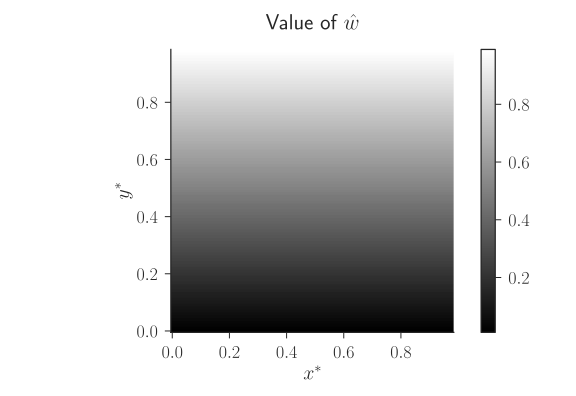
\includegraphics[width=\textwidth]{w-hat-empirical-01-marginal}
\caption{
    Estimates for $\hat{w}$ when computing $(\hat{x}, \hat{y}, \hat{w})$ using basin-hopping \cite{Wales1997} optimizing \eqref{eq:marginal_likelihood}.
}
\label{fig:bl-general-marginal}
\end{figure}

\begin{figure}
\centering
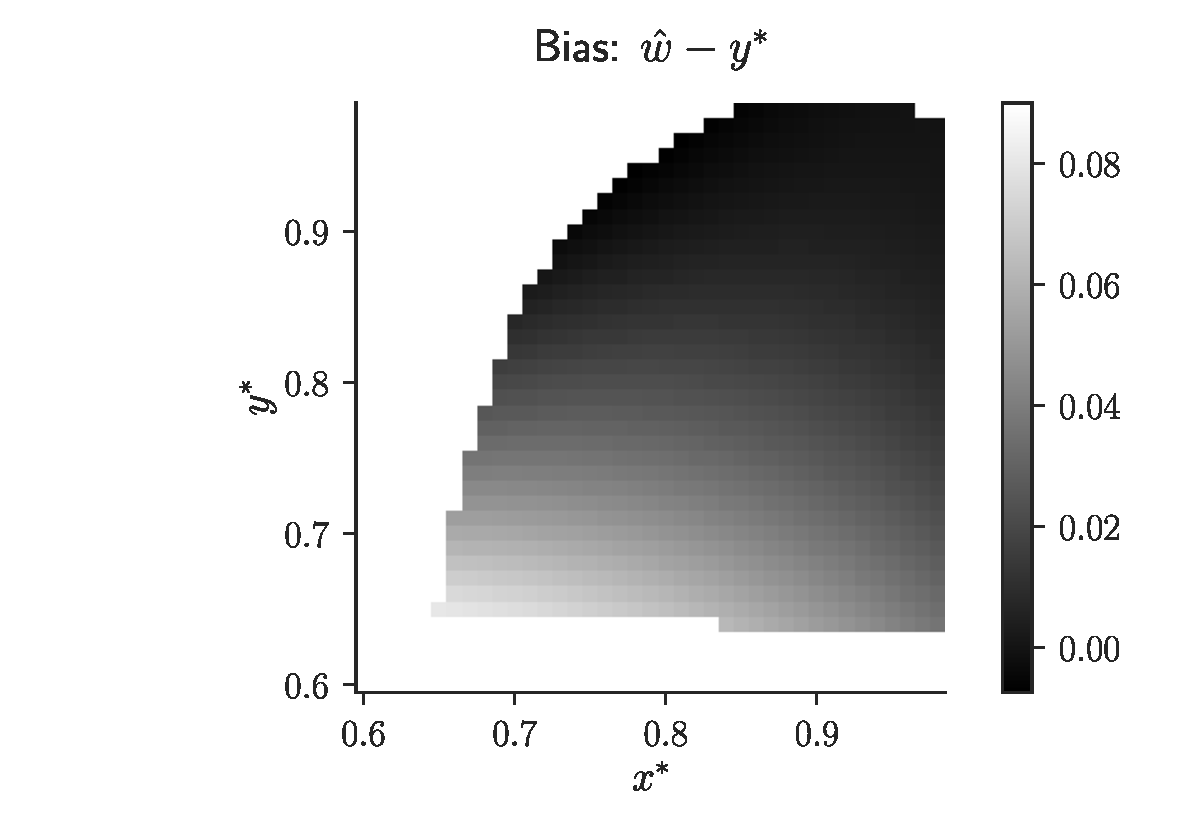
\includegraphics[width=\textwidth]{w-hat-empirical-01-bias}
\caption{
    Estimates for $\hat{w}-y^*$ when computing $(\hat{x}, \hat{y}, \hat{w})$ using basin-hopping \cite{Wales1997} optimizing \eqref{eq:marginal_likelihood}.
    Plot focuses on $0.6 < x^*, y^* < 1$ where $\hat{w}$ is estimated to be a value different from 1.
}
\label{fig:bl-general-bias}
\end{figure}

